
%----------------------------------------------------------------------------------------
%	PACKAGES AND OTHER DOCUMENT CONFIGURATIONS
%---------------------------------------------------------------------------------------

\documentclass[11pt]{scrartcl} % Font size
\newcommand{\comment}[1]{}
%%%%%%%%%%%%%%%%%%%%%%%%%%%%%%%%%%%%%%%%%
% Wenneker Assignment
% Structure Specification File
% Version 2.0 (12/1/2019)
%
% This template originates from:
% http://www.LaTeXTemplates.com
%
% Authors:
% Vel (vel@LaTeXTemplates.com)
% Frits Wenneker
%
% License:
% CC BY-NC-SA 3.0 (http://creativecommons.org/licenses/by-nc-sa/3.0/)
% 
%%%%%%%%%%%%%%%%%%%%%%%%%%%%%%%%%%%%%%%%%

%----------------------------------------------------------------------------------------
%	PACKAGES AND OTHER DOCUMENT CONFIGURATIONS
%----------------------------------------------------------------------------------------

\usepackage{amsmath, amsfonts, amsthm} % Math packages

\usepackage{listings} % Code listings, with syntax highlighting

\usepackage[english]{babel} % English language hyphenation

\usepackage{graphicx} % Required for inserting images
\graphicspath{{Figures/}{./}} % Specifies where to look for included images (trailing slash required)

\usepackage{booktabs} % Required for better horizontal rules in tables

\numberwithin{equation}{section} % Number equations within sections (i.e. 1.1, 1.2, 2.1, 2.2 instead of 1, 2, 3, 4)
\numberwithin{figure}{section} % Number figures within sections (i.e. 1.1, 1.2, 2.1, 2.2 instead of 1, 2, 3, 4)
\numberwithin{table}{section} % Number tables within sections (i.e. 1.1, 1.2, 2.1, 2.2 instead of 1, 2, 3, 4)

\setlength\parindent{0pt} % Removes all indentation from paragraphs

\usepackage{enumitem} % Required for list customisation
\setlist{noitemsep} % No spacing between list items

%----------------------------------------------------------------------------------------
%	DOCUMENT MARGINS
%----------------------------------------------------------------------------------------

\usepackage{geometry} % Required for adjusting page dimensions and margins

\geometry{
	paper=a4paper, % Paper size, change to letterpaper for US letter size
	top=2.5cm, % Top margin
	bottom=3cm, % Bottom margin
	left=3cm, % Left margin
	right=3cm, % Right margin
	headheight=0.75cm, % Header height
	footskip=1.5cm, % Space from the bottom margin to the baseline of the footer
	headsep=0.75cm, % Space from the top margin to the baseline of the header
	%showframe, % Uncomment to show how the type block is set on the page
}

%----------------------------------------------------------------------------------------
%	FONTS
%----------------------------------------------------------------------------------------

\usepackage[utf8]{inputenc} % Required for inputting international characters
\usepackage[T1]{fontenc} % Use 8-bit encoding

\usepackage{fourier} % Use the Adobe Utopia font for the document

%----------------------------------------------------------------------------------------
%	SECTION TITLES
%----------------------------------------------------------------------------------------

\usepackage{sectsty} % Allows customising section commands

\sectionfont{\vspace{6pt}\centering\normalfont\scshape} % \section{} styling
\subsectionfont{\normalfont\bfseries} % \subsection{} styling
\subsubsectionfont{\normalfont\itshape} % \subsubsection{} styling
\paragraphfont{\normalfont\scshape} % \paragraph{} styling

%----------------------------------------------------------------------------------------
%	HEADERS AND FOOTERS
%----------------------------------------------------------------------------------------

\usepackage{scrlayer-scrpage} % Required for customising headers and footers

\ohead*{} % Right header
\ihead*{} % Left header
\chead*{} % Centre header

\ofoot*{} % Right footer
\ifoot*{} % Left footer
\cfoot*{\pagemark} % Centre footer
 % Include the file specifying the document structure and custom commands
%\usepackage{flafter}
\usepackage[section]{placeins}
\usepackage{caption}
\usepackage{float}
%----------------------------------------------------------------------------------------
%	TITLE SECTION
%----------------------------------------------------------------------------------------

\title{	
	\normalfont\normalsize
	\textsc{Rutgers University, New Brunswick}\\ % Your university, school and/or department name(s)
	\vspace{25pt} % Whitespace
	\rule{\linewidth}{0.5pt}\\ % Thin top horizontal rule
	\vspace{20pt} % Whitespace
	{\huge Minesweeper}\\ % The assignment title
	\vspace{12pt} % Whitespace
	\rule{\linewidth}{2pt}\\ % Thick bottom horizontal rule
	\vspace{12pt} % Whitespace
}

\author{\LARGE Eshaan Gandhi} % Your name

\date{\normalsize\today} % Today's date (\today) or a custom date

\begin{document}

\maketitle % Print the title

\section{Representation}
I used different representation for different parts of the project.
For part 1 - I took a more object oriented programming design. While, for part 2 I had a more functional design. 
\subsection{Hidden Board}
In terms of the board that is native to the enthronement, I had a very simple board. It is just a numpy array. This numpy 2-d array was first populated with mines and then populated with the clues. This information in the array is hidden away from the user and can only be gathered through a query function. To assure that no cheating can be done by me, as soon as anyone queries a mine, the score immediately drops in a global variable. This is then encapsulated away in a function away from the user, in the environment.py script. 

\subsection{Player Board - part 1}
Now we come to the information that is available to the user. To do this I created a cell python script that had all the attributes one could have created when an object of the type was created. \\
The attributes of the cell python script are as follows:
\begin{itemize}[leftmargin = *]
\item Whether or not it is a mine or safe (or currently covered)
\item If safe, the number of mines surrounding it indicated by the clue
\item The number of safe squares identified around it
\item The number of mines identified around it.
\item The number of hidden squares around it.
\end{itemize}

I then created a board to individually store the knowledge base. This knowledge base was populated as we went. Every cell contained information that only concerned itself and not the others. There was no use of information from others to make decisions. Every cell contained the above mentioned information, that was continuously updated. 

\subsection{Agent - part 1}
The agent for part 1 was very basic and only opened obvious safe space, and marked obvious mines. This agent only looked at a single cell and try to derive conclusions from that. It did not "learn" from information around it.\\
The agent could learn see all the information of a particular state if it was already queried. Non queried cells would not allow the agent to see abstracted information.  
\comment{
It followed the following algorithm (given by Prof Cowan)

}

\subsection{Player Board - part 2}
The player board for part 2 is very basic. It is a numpy array that just holds the clues. The knowledge base for this part is the complex part. The knowledge base for part 2 was designed to be accessed by something like a computer, with a lot of computational power. Thus it is represented in lists and sets that can be looked up and iterated through easy, but to the naked eye it is very haphazard and drawing relations can be hard. \\
The knowledge base is represented using sets and arrays. The main knowledge base is a list of dictionaries. Every dictionary represents a proposition. An example entry in the knowledge base looks like this:
\begin{center}
$2.0:{A, B, C, D, E, F, G}$\\
$1.0:{B, C, D}$ 
\end{center}
This basically means that out of A, B, C, D, E, F, G two of them have mines. Out of B, C, D 1 of them has a mine. We can also infer more information from these propositions, but more on that later. \\
We also have a couple of sets that store the safe cells and the mines to be used to trim the knowledge base. 

\subsection{Agent - part 1}
The agent for part 1 has access to a very basic board where it keeps track of all the clues and mines (either flagged or mistakenly) exploded. It also has access to knowledge bases that are used to infer mines that are safe and mines that are not. Again, the agent could learn see all the information of a particular state if it was already queried. Non queried cells would not allow the agent to see abstracted information. The knowledge base is only added to if a query is made. 

\section{Inference}
\subsection{Basic Agent}
The rules for inference for the basic and advanced models were mostly the same. I started out by the basic algorithm that is trivial and also provided by Dr. Cowan. 
\begin{itemize}[leftmargin = *]
\item If, for a given cell, the total number of mines (the clue) minus the number of revealed mines is the number ofhidden neighbors, every hidden neighbor is a mine.
\item If, for a given cell, the total number of safe neighbors (8 - clue) minus the number of revealed safe neighbors isthe number of hidden neighbors, every hidden neighbor is safe.
\item If a cell is identified as safe, reveal it and update your information.
\item If a cell is identified as a mine, mark it and update your information.
\item If no hidden cell can be conclusively identified as a mine or safe, pick a cell to reveal at random.
\end{itemize} 

* The basic model follows this exact algorithm, and surprisingly does pretty well. Comparison and analysis will be done in another section. 

\subsection{Advance Agent}
The advanced agent does the same thing as the basic agent but does additional inferences in the knowledge base. Going back to the example that was given earlier.
\begin{center}
$2.0:{A, B, C, D, E, F, G}$\\
$1.0:{B, C, D}$ 
\end{center}
We see that {B, C, D} is a subset of {A, B, C, D, E, F, G}. This implies that {A, B, C, D, E, F, G} - {B, C, D} will have $2-1=1$ mine. Thus we have a new entry in the knowledge base that goes as follows: $1.0:{A, E, F, G}$. Thus by collecting new information like this we keep going until we hit the base cases as mentioned before. We also identify a safe cell and remove it from the knowledge base, as it slows down our decision making. 

\section{Decisions}
\subsection{Basic Agent}
The program actually goes through the whole board and checks if any of the basic conditions are fulfilled. If it cannot find it, it just picks randomly.
\subsection{Advanced Agent}
So the advanced agent goes through the whole knowledge base and tries to get more information before it can look for the base cases. If even after trying to find subsets it cannot it opens any cell on random. 

PS: This can be improved using probability where it does not randomly open spaces. 
\section{Performance - 1}
The step by step was is in a text file attached to the submission. Sorry for the inconvenience. 
\section{Performance - 2}
So I chose a 10X10 board for my agents to play. I start out with 8 mines and then increase it by 2 everytime until I have 26 mines in a 10X10 board. I then ran each agent a 100 times to get a good average for the success rate. The table and graph below capture my results.\\
The score is calculated by $\frac{mines - mines\ exploded}{mines} * 100$
\begin{table}[H]
\begin{tabular}{|l|l|l|l|}
\hline
Iterations & Mine - Density & Score agent 1 & Score agent 2 \\ \hline
100        & 0.08           & 97.125        & 97.25         \\ \hline
100        & 0.1            & 97.4          & 96.5          \\ \hline
100        & 0.12           & 94.5          & 95.75         \\ \hline
100        & 0.14           & 91.00         & 95.43         \\ \hline
100        & 0.16           & 88.69         & 92.65         \\ \hline
100        & 0.18           & 83.39         & 91.89         \\ \hline
100        & 0.20           & 80.60         & 89.35         \\ \hline
100        & 0.22           & 75.05         & 85.55         \\ \hline
100        & 0.24           & 72.05         & 82.71         \\ \hline
100        & 0.26           & 67.15         & 80.58         \\ \hline
\end{tabular}
\end{table}
We also see in the graph below how they compare to each other
\begin{figure}[H]
\begin{center}
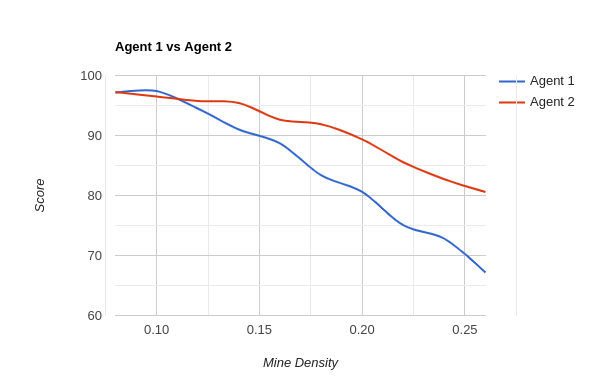
\includegraphics[scale=.75]{Figures/line-graph.png}
\end{center}
\end{figure}

We see that agent 2 does a lot better when there is a higher density. The graph definitely makes sense intuitively. It becomes hard when you have to make a lot of random moves that are not based in logic. That can happen a lot if you consider agent 1's strategy during the first few attempts when not a lot is known about the board. The simple algorithm is good when there are not a lot of mines and it can expand a lot of cells just by seeing a zero. This is not the case when the mine density is high. 

\section{Efficiency}
As far as efficiency is concerned, this is a very computationally expensive task. We have to constantly check if there is any information in our knowledge base that we can use. This is $O(n^2)$ every single time we have to make a move. This causes the program to slow down very quickly as the complexity increases. This can be improved if we use the correct data structures for our knowledge base. If we use sets effectively we can look up in constant time. 
\subsection{Agent 2}
The subset function is especially computationally and space expensive. Since we use arrays and dictionaries, for a big enough data set, space will be very hard to optimize. The subset function goes through the whole knowledge base and compares each and every entry against each other to draw inferences. 

\section{Citations}
https://cs50.harvard.edu/ai/2020/projects/1/minesweeper/\\
Idea taken from there for inference
\end{document}